\documentclass[a4paper,12pt]{report}
\usepackage[utf8]{inputenc}


\usepackage{tikz}
\usetikzlibrary{calc}
\usepackage{subcaption}

\begin{document}

\thispagestyle{empty}

\begin{figure}[h!]
		\centering
		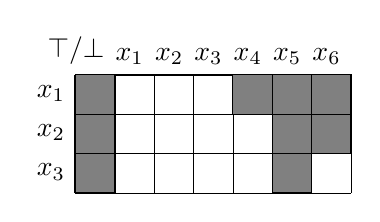
\begin{tikzpicture}
		%grid outline
		\draw[step=0.5cm,black,very thin] (0,0) grid (3.5,1.5);
		
		%indexes
		\draw[thick] (0,1.5) -- (0.5,1.5) node[anchor=south east] {$\top$/$\bot$};
		\draw[thick] (0.5,1.5) -- (1,1.5) node[anchor=south east] {$x_{1}$};
		\draw[thick] (1,1.5) -- (1.5,1.5) node[anchor=south east] {$x_{2}$};
		\draw[thick] (1.5,1.5) -- (2,1.5) node[anchor=south east] {$x_{3}$};
		\draw[thick] (2,1.5) -- (2.5,1.5) node[anchor=south east] {$x_{4}$};
		\draw[thick] (2.5,1.5) -- (3,1.5) node[anchor=south east] {$x_{5}$};
		\draw[thick] (3,1.5) -- (3.5,1.5) node[anchor=south east] {$x_{6}$};
	
	    %representatives
	    \draw[thick] (0,1) -- (0,1.5) node[anchor=north east] {$x_{1}$};
		\draw[thick] (0,0.5) -- (0,1) node[anchor=north east] {$x_{2}$};
		\draw[thick] (0,0) -- (0,0.5) node[anchor=north east] {$x_{3}$};
		
		%bits
		\filldraw[black!50!white, draw=black] (0,1) rectangle (0.5,1.5);
		\filldraw[black!50!white, draw=black] (2,1) rectangle (2.5,1.5);
		\filldraw[black!50!white, draw=black] (2.5,1) rectangle (3,1.5);
		\filldraw[black!50!white, draw=black] (3,1) rectangle (3.5,1.5);
		
		\filldraw[black!50!white, draw=black] (0,0.5) rectangle (0.5,1);
		\filldraw[black!50!white, draw=black] (2.5,0.5) rectangle (3,1);
		\filldraw[black!50!white, draw=black] (3,0.5) rectangle (3.5,1);
		
		\filldraw[black!50!white, draw=black] (0,0) rectangle (0.5,0.5);
		\filldraw[black!50!white, draw=black] (2.5,0) rectangle (3,0.5);
	
		\end{tikzpicture}
		\caption{The $EC$ structure.}
		\label{fig:ec_struct_0}
	\end{figure}

\end{document}
